\begin{question}[topic=suites]
  On donne la suite $(u_n)$ définie par $\forall n\in \mathbf{N},
  u_{n+1} = \frac{1}{\sqrt{2}}u_{n} + 1$ et $u_0 = 0$.
  \begin{enumerate}
    \item La suite $(u_n)$ est ici définie par $u_{n+1} = f(u_n)$. Quelle
      condition respecte la fonction $f$ ici pour pouvoir dire si $u_n$
      converge vers $\ell$, alors $f(\ell) = \ell$ ?
    \item Calculer la valeur de $\ell$.
    \item Soit la suite $(v_n)$ définie par $\forall n\in \mathbf{N}, v_n
      = u_n - \frac{2}{2 - \sqrt{2}}$.
      \begin{enumerate}
        \item Montrer que $(v_n)$ est décroissante.
        \item En admettant que la suite $(v_n)$ est minorée par 0, que
          peut-on dire de la convergence de cette suite ?
        \item En déduire la limite de la suite $(u_n)$.
      \end{enumerate}
  \end{enumerate}
\end{question}

\begin{question}[topic=probabilités]
  On considère un sac opaque contenant trois billes rouges et deux billes
  bleues indiscernables au toucher.

  On effectue un tirage sans remise.

  \begin{enumerate}
    \item Quelle est la probabilité de tirer une bille bleue, puis une
      bille rouge ?
    \item Quelle est la probabilité de tirer une bille rouge puis une
      bille bleue.
    \item Les événements «tirer une bille bleue puis une bille rouge» et
      «tirer une bille rouge puis une bille bleue» sont ils indépendants.
  \end{enumerate}
\end{question}

\begin{question}[topic=complexes]
  On désigne par $A$ et $B$ les points du plan complexe d'affixe $z_A = 1$
  et $z_B = i$.
  \begin{enumerate}
    \item Déterminer l'ensemble des points $M$ d'affixe $z$ du plan
      complexe tels que $\left\lvert z - 1 \right\rvert = \left\lvert z -
      i \right\rvert$.
    \item Montrer que l'ensemble des points $M$ d'affixe $z$ du plan
      complexe tel que $\frac{z - i}{z -1}$ soit un imaginaire pur est un
      cercle de diamètre $[AB]$ privé du point $A$.
    \item Écrire une équation permettant de trouver les points
      d'intersection de la droite et du cercle. On ne demande pas de la
      résoudre ici.
  \end{enumerate}
\end{question}

\begin{question}[topic=fonction]
  On considère la fonction de la variable réelle $x$ définie sur
  l'ensemble des nombres réels positifs par $f(x) = \frac{2x - \sqrt{x}}{2
  + \sqrt{x}}$.

  \begin{enumerate}
    \item Montrer que $f$ est dérivable sur $\left]0 ; +\infty\right[$ et
      que $f'(x) = \frac{ x + 4\sqrt{x} - 1}{\sqrt{x}(2 + \sqrt{x})^2}$
    \item Résoudre l'équation $X^2 + 4X - 1 =0$ en déduire le signe de
      $f'(x)$.
    \item Dresser le tableau de variation complet de $f$.
  \end{enumerate}
\end{question}

\begin{question}[topic=géométrie]
  On considère la droite $\Delta$ de représentation paramétrique \[ \Delta
    : \left\lbrace \begin{array}{lr} x = 1 - 4t & \\ y = 3 + t & t\in
  \mathbf{R} \\ z = 1 - t & \end{array}\right. \]

  \begin{enumerate}
    \item Donner un point et un vecteur directeur de $\Delta$.
    \item Le point $M (-3;4;1)$ appartient-il à la droite $\Delta$.
    \item Proposer une autre représentation paramétrique de cette droite.
  \end{enumerate}
\end{question}

\begin{question}[topic=loi_continue]
  En rentrant de soirée, Léo sait qu'il va arriver dans la station de
  métro la plus proche entre 1h et 1h30. On fait l'hypothèse que son heure
  d'arrivée suit une loi uniforme. Depuis minuit, il passe un métro toutes
  les 20 minutes dans cette station. Quelle est la probabilité que Léo
  attente :
  \begin{enumerate}
    \item moins de 5 minutes ;
    \item plus d'un quart d'heure.
  \end{enumerate}

  On rappelle que :
  \begin{itemize}
    \item pour une loi à densité $f$ continue, $P(X \leq x) =
      \int_{-\infty}^x f(t) \mathrm{d}\,t$ ;
    \item la densité de probabilité de la loi uniforme entre $a$ et $b$
      est $f : \left\lbrace \begin{array}{lr} \frac1{b-a} & x \in ]a;b[
    \\ 0 & \text{sinon}\end{array}\right.$
  \end{itemize}
\end{question}

\begin{question}[topic=exponentielle]
  Question de cours : Démontrer que s'il existe une fonction $f$ telle que
  pour tout $x$ réel, $f'(x) = f(x)$ et $f(0) = 1$, alors cette fonction
  est unique.

  Démontrer de plus que $f(a+b) = f(a)f(b)$.
\end{question}

\begin{question}[topic=loi_exponentielle]
  Question de cours : Démontrer que la loi exponentielle (définie par la
  densité de probabilité $f(t) = \lambda e^{-\lambda t}$) définie bien une
  loi sans mémoire, c'est-à-dire que pour $t$ et $s$ deux réels positifs,
  $P_{T>s}(T > s+t) = P(T > t)$.
\end{question}

\begin{question}[topic=recurrence]
  Discuter (et démontrer évenutellement) pour des valeurs de $n$ entières
  l'inégalité $5^n \geqslant 4^n + 3^n$.
\end{question}

\begin{question}[topic=géométrie]
  Question de cours : démontrer qu'une droite $\mathcal{D}$ est
  parallèle à un plan $\mathcal{P}$ si et seulement si elle est parallèle
  à deux droites sécantes de ce plan.
\end{question}

\begin{question}[topic=suite]
  On considère la suite numérique $(u)$ défine par $u_0 = \frac12$ et pour
  tout $n$ entier naturel, $u_{n+1} = \frac{3u_n}{1 + 2u_n}$.

  \begin{enumerate}
    \item Démontrer, par récurrence, que la suite est minorée par 0.
    \item On admet que la suite est majorée par 1. Montrer qu'elle est
      croissante. Justifier alors qu'elle converge.
    \item Soit $v_n = \frac{u_n}{1 - u_n}$. Montrer que $v_n$ est une
      suite géométrique de raison 3.
    \item On admet que $u_n = \frac{3_n}{3^n + 1}$. Donner sa limite.
  \end{enumerate}
\end{question}

\begin{question}[topic=loi_continue]
  Fred a remarqué qu'il mettait en moyenne 20 minutes pour aller à son
  lycée. On considère que sa durée de trajet, modélisée par une variable
  aléatoire $D$ suit une loi normale de paramètes $\mu = 20$ et $\sigma$
  inconnu.

  \begin{enumerate}
    \item En partant à 7h40 pour 8h, quelle est la probabilité qu'il
      arrive à l'heure ?
    \item Voyant qu'il est trop souvent en retard, il décide de partir à
      7h30. La probabilité de retard est désormais de 0,0228.

      Déterminer $\sigma$.
    \item À quelle heure doit-il partir pour arriver à l'heure avec une
      probabilité de 99\% ?
  \end{enumerate}
\end{question}

\begin{question}[topic=exponentielle]
  Question de cours : Donner puis démontrer
  $\lim_{x\to+\infty}\frac{e^x}x$.
\end{question}

\begin{question}[topic=cos:complexes]
  Calcul de $\cos\frac{2\pi}{5}$

  \begin{enumerate}
    \item Montrer que tout nombre complexe $z\neq 1$, $1 + z + z^2 + z^3 +
      z^4 = \frac{1 - z^5}{1 - z}$.
    \item Démontrer alors que pour $z_0 = e^{i\frac{2\pi}5}$, $\left(z_0^2
      + \frac1{z_0^2} \right) + \left(z_0 + \frac1{z_0}\right) + 1 = 0$
    \item Montrer que $\left(z_0^2 + \frac1{z_0^2} \right) = \left(z_0 +
      \frac1{z_0}\right)^2 - 2$.
    \item On admet que
      \begin{itemize}
        \item $z_0 + \frac1{z_0} = 2\cos\frac{2\pi}5$ ;
        \item si on pose $X = 2\cos\frac{2\pi}5$, alors $X$ est solution
          de $X^2 + X - 3 = 0$.
      \end{itemize}
      Calculer la valeur de $\cos\frac{2\pi}5$.
  \end{enumerate}
\end{question}

\begin{question}[topic=intégrale]
  Question de cours : Démontrer que si $F$ est une primitive de $f$ sur un
  intervalle $[a;b]$ alors $f$ admet une infinité de primitive de la forme
  $x\mapsto F(x) + k,\ \in\mathbf{R}$.
\end{question}

\begin{question}[topic=géométrie]
  On donne, dans un repère orthnormé l'équation paramétrique suivante :
  \[ \left\lbrace \begin{array}{lr}
      x = 1 - s + 4t &                                 \\
      y = 2 + 2s -t  & s\in\mathbf{R}, t\in \mathbf{R} \\
      z = -1 +s + 2t &                                 \\
  \end{array}\right.\]

  \begin{enumerate}
    \item Cette représentation paramétrique définit-elle un plan ?
    \item Déterminer un vecteur normal à ce plan.
    \item En déduire une équation cartésienne.
  \end{enumerate}
\end{question}

\begin{question}[topic=probabilités]
  Question de cours : Démontrer que si $A$ et $B$ sont indépendants, alors
  $A$ et $\overline{B}$ le sont aussi.
\end{question}

\begin{question}[topic=fonction]
  On considère la fonction $f$ définie sur $]0;+\infty[$ par $f(x) = \ln x
  + x^2$.

  \begin{enumerate}
    \item Déterminer les limites de $f$ aux bornes de son intervalle de
      définition.
    \item Calculer $f'(x)$ et étudier son signe.
    \item Dresser le tableau de variation de $f$.
    \item Montrer que l'équation $f(x) = 0$ admet une unique solution
      $\alpha$ dans l'intervalle $]0;+\infty[$.
    \item Donner une valeur approchée de $\alpha$ à $10^{-2}$ près.
  \end{enumerate}
\end{question}

\begin{question}[topic=nombres_complexes]
  Question de cours : montrer les trois affirmations suivantes :
  \begin{itemize}
    \item Affirmation 1 : $z + \overline{z} = 2\Re(z)$
    \item Affirmation 2 : $z - \overline{z} = 2i\Im(z)$
    \item Affirmation 3 : $z \times \overline{z} = \lvert z \rvert^2$
  \end{itemize}
\end{question}

\begin{question}[topic=fonction]
  Soit la fonction $f$ définie sur $[-1;1]$ par $f(x) = (1-x^2)e^x$.

  \begin{enumerate}
    \item Calculer la dérivée de $f$ et en déduire les variations de la
      fonctions $f$. Préciser les valeurs $f(-1)$ et $f(1)$.
    \item Donner la valeur de $x_{\max}$ pour laquelle le maximum est
      atteint et donner $f(x_{\max})$.
    \item On donne $f''(x) = \left(-x^2-4x-1\right)e^{x}$. Montrer que
      $f(x) - 2f'(x) + f''(x) = - 2e^x$.

      En déduire $\int_{-1}^1 f(x) \mathrm\,x$.
    \item Interpréter géométriquement ce résultat.
  \end{enumerate}
\end{question}

\begin{question}[topic=suite]
  On considère la suite $(w_n)$ définie par $w_0=2$ et
  $w_n=\dfrac15w_{n-1}+\dfrac12$ pour tout entier $n\geqslant1$.

  Montrer que $w_n=\dfrac{11}{8}\left(\dfrac{1}{5}\right)^n+\dfrac{5}{8}$
  pour tout $n\geqslant0$.
\end{question}

\begin{question}[topic=suite]
  On considère la suite définie par $u_1=8$ et
  ${u_{n+1}=\dfrac{1}{2}u_n+2n-3}$ pour tout $n\in\N^*$.
  \begin{enumerate}
    \item Montrer que $u_n\geqslant n$ pour tout $n\geqslant 4$.
    \item En déduire $\displaystyle \lim_{n\rightarrow +\infty} u_n$.
  \end{enumerate}
\end{question}

\begin{question}[topic=fonction]
  La fonction $f$ définie sur $\mathbb{R}$ par :
  \[f(x)=\left\{\begin{array}{@{}ll}
        2+\sqrt{5} & \text{si~} x\leqslant0 \\
        \sqrt{9+4\sqrt{5}} & \text{si~} x>0 \\
  \end{array}\right..\]
  est-elle continue en 0 ?
\end{question}

\begin{question}[topic=fonction]
  \begin{enumerate}
    \item Soit $n\in\mathbb{N}^*$  et $f$ la fonction définie sur
      $\mathbb{R}$ par : \[f(x)=(1+x)^n-1-nx.\]
      Établir le sens de variation  de $f$ sur $[-1~;~+\infty[$.
    \item
      \begin{enumerate}
        \item Établir \textbf{l'inégalité de Bernoulli} :
          \[(1+x)^n\geqslant 1+nx\]
          pour tout $n\in\mathbb{N}^*$ et tout $x\in[-1~;~+\infty[$.
        \item Pour quelle(s) valeur(s) de $x$ a-t-on l'égalité ?
      \end{enumerate}
  \end{enumerate}
\end{question}

\begin{question}[topic=fonction]
  Soit la fonction $f$ définie sur $[0~;~+\infty[$ par :
  \[f(x)=\dfrac{2x-\sqrt{x}}{2+\sqrt{x}}.\]
  \begin{enumerate}
    \item Montrer que $f$ est dérivable sur $]0~;~+\infty[$ et que :
      \[f'(x)=\dfrac{x+4\sqrt{x}-1}{\sqrt{x}\left(2+\sqrt{x}\right)^2}.\]
    \item Résoudre l'équation $X^2+4X-1=0$.\par
      En déduire le signe de $f'(x)$.
    \item Dresser le tableau de variation complet de $f$.
  \end{enumerate}
\end{question}

\begin{question}[topic=exponetielle]
  Soit $f$ la fonction définie pour tout $x\in\left[0~;~1\right]$ par :
  \[f(x)=2x-2e^{-x}+e^{-1}.\]
  \begin{enumerate}
    \item Dresser le tableau de variation de $f$ sur $\left[0~;~1\right]$.
    \item Démontrer que la fonction $f$ s'annule une fois et une seule sur
      l'intervalle $\left[0~;~1\right]$ en un réel $\alpha$.\par
      Donner la valeur de $\alpha$ arrondie au centième.
  \end{enumerate}
\end{question}

\begin{question}[topic=logarithme]
  On considère la fonction $f$ définie sur $ \left] 0 \, ;+\infty \right[ $
  par $f(x)=x \ln x$.
  \begin{enumerate}
    \item Étudier les limites de $f$ en 0 et en $+\infty$.
    \item Pour tout réel $x>0$, calculer $f^{\prime}(x)$.
    \item Étudier le signe de  $f^{\prime}(x)$ et en déduire les variations
      de $f$.
    \item En déduire que $f$ admet un minimum sur $\left] 0 \,
      ;+\infty\right[ $ que l'on précisera.
\end{enumerate}
\end{question}

\begin{question}[topic=logarithme]
  En 2015, la population d'une ville compte \\250 000 habitants. Chaque
  année, cette population diminue de $2 \, \%$. À partir de quelle année la
  population passera-t-elle au-dessous de 100 000 habitants?
\end{question}

\begin{question}[topic=logarithme]
  Déterminer le plus petit entier naturel $n$ tel que :
  \[ 1+5+5^2+...+5^n \geqslant 10^9. \]
\end{question}

\begin{question}[topic=integration]
  On souhaite calculer l'intégrale suivante :
  \[ I = \int_0^1 \dfrac{x}{x+1}\,\mathrm{d}x. \]
  \begin{enumerate}
    \item Expliquer pourquoi $f : x \mapsto \dfrac{x}{x+1}$ ne correspond à
      aucune forme de dérivée connue.
    \item En remarquant que $x = x + 1 - 1$ , démontrer que pour tout $x
      \neq -1$, $f(x)$ peut s'écrire sous la forme \[f(x) = \alpha+
      \dfrac{\beta}{x+1}\] où $\alpha$ et $\beta$ sont deux réels à
      déterminer.
    \item En déduire que $I = 1 - \ln(2)$.
  \end{enumerate}
\end{question}

\begin{question}[topic=complexes]
  On pourra utiliser comme prérequis que pour tous nombres complexes $z_1$
  et $z_2$ on a : $$\overline{z_1\times z_2}=\overline{z_1}\times
  \overline{z_2}.$$
  \begin{enumerate}
    \item Démontrer par récurrence que pour tout entier naturel $n\geqslant
      1$ on a $\overline{z^n}=\overline{z}^n$
    \item En déduire que pour tout entier naturel $n\geqslant 1$ et pour
      tout nombre complexe $z$ : $z^n+\overline{z}^n$ est un nombre réel.
    \item Démontrer que pout tout entier naturel $n$ le complexe
      $(2-i)^{2n}+(3-4i)^n$ est un nombre réel.
  \end{enumerate}
\end{question}

\begin{question}[topic=geometrie]
  On considère le cube suivant, d'arête 1, où $I$ et $J$ sont les milieux
  respectifs de $[EH]$ et $[FG]$. Soit $M$ un point appartenant à $[IJ]$.

  \begin{center}
    \def \dx {-0.4}
    \def \r {0.3}
    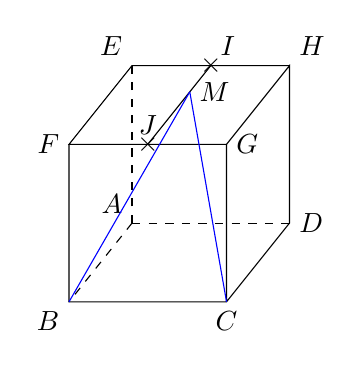
\begin{tikzpicture}[scale=2]
      %points
      \coordinate (A) at (0,0); \draw (A) node[above left] {$A$};
      \coordinate (B) at (\dx,-0.5); \draw (B) node[below left] {$B$};
      \coordinate (C) at (1+\dx,-0.5); \draw (C) node[below] {$C$};
      \coordinate (D) at (1,0); \draw (D) node[right] {$D$};
      \coordinate (E) at (0,1); \draw (E) node[above left] {$E$};
      \coordinate (F) at (\dx,0.5); \draw (F) node[left] {$F$};
      \coordinate (G) at (1+\dx,0.5); \draw (G) node[right] {$G$};
      \coordinate (H) at (1,1); \draw (H) node[above right] {$H$};
      \coordinate (I) at (0.5,1); \draw (I) node[above right] {$I$}; \draw (I) node {$\times$};
      \coordinate (J) at (0.5+\dx,0.5); \draw (J) node[above] {$J$}; \draw (J) node {$\times$};
      \coordinate (M) at (0.5+\dx/3,5/6); \draw (M) node[right] {$M$};
      %arêtes
      \draw (F)--(B)--(C)--(D)--(H)--(G)--(C); \draw (G)--(F)--(E)--(H);
      \draw[dashed] (A)--(B); \draw[dashed] (A)--(D); \draw[dashed] (A)--(E);
      %IJ, MB et MC
      \draw[thin] (I)--(J);
      \draw[color=blue] (M)--(B); \draw[color=blue] (M)--(C);
    \end{tikzpicture}
  \end{center}

  \begin{enumerate}
    \item \begin{enumerate}
      \item Démontrer que pour $M \neq J$, les triangles $MJB$ et $MJC$ sont rectangles en $J$.
      \item En déduire que $MB = MC$.
      \item En déduire que $\vv{MB} \cdot \vv{MC} = MB^2 - \dfrac{1}{2}$.
    \end{enumerate}

  \item Déterminer la ou les positions du point $M$ pour que $\vv{MB} \cdot \vv{MC}=1$.
\end{enumerate}
\end{question}

\begin{question}[topic=géométrie]
  Soit $SABC$ un tétraèdre de tel que les triangles $ABC$ et $SBC$ soient
  isocèles respectivement en $A$ et $S$ :
  \begin{center}
    %\includegraphics[scale=0.3]{./images/tetra_triangles_isoceles.eps}
    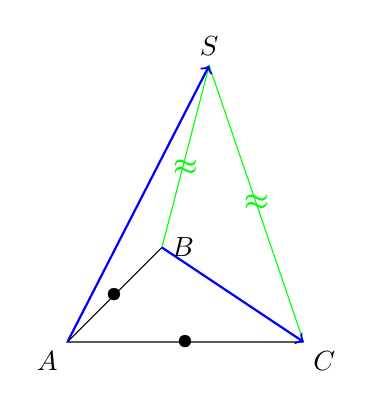
\begin{tikzpicture}[scale=3]
      %points
      \coordinate (A) at (0,0); \draw (A) node[below  left] {$A$};
      \coordinate (C) at (1,0); \draw (C) node[below right] {$C$};
      \coordinate (B) at (0.4,0.4); \draw (B) node[right] {$B$};
      \coordinate (S) at (0.6,1.17); \draw (S) node[above] {$S$};
      %segments
      \draw[color=black] (C)--(A)--(B);
      \draw[color=green] (B)--(S)--(C);
      \draw[color=blue, ->, thick] (B)--(C);
      \draw[color=blue, ->, thick] (A)--(S);
      %codage
      \draw[color=black] (0.5,0) node {{\boldmath $\bullet$}};
      \draw[color=black] (0.2,0.2) node {{\boldmath $\bullet$}};
      \draw[color=green] (0.5,0.74) node {{\boldmath $\approx$}};
      \draw[color=green] (0.8,0.59) node {{\boldmath $\approx$}};
    \end{tikzpicture}
  \end{center}

  Démontrer que $\vv{AS} \cdot \vv{BC} = 0$.
\end{question}

\begin{question}[topic=géométrie]
  On considère un cube $ABCDEFGH$ de côté 1 et de centre $O$.
  \begin{center}
    \def \dx {-0.4}
    \def \r {0.3}
    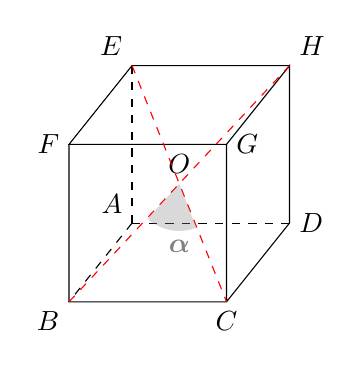
\begin{tikzpicture}[scale=2]
      %points
      \coordinate (A) at (0,0); \draw (A) node[above left] {$A$};
      \coordinate (B) at (\dx,-0.5); \draw (B) node[below left] {$B$};
      \coordinate (C) at (1+\dx,-0.5); \draw (C) node[below] {$C$};
      \coordinate (D) at (1,0); \draw (D) node[right] {$D$};
      \coordinate (E) at (0,1); \draw (E) node[above left] {$E$};
      \coordinate (F) at (\dx,0.5); \draw (F) node[left] {$F$};
      \coordinate (G) at (1+\dx,0.5); \draw (G) node[right] {$G$};
      \coordinate (H) at (1,1); \draw (H) node[above right] {$H$};
      \coordinate (O) at ({(1+\dx)/2},0.25); \draw (O) node[above] {$O$};
      %arêtes
      \draw (F)--(B)--(C)--(D)--(H)--(G)--(C); \draw (G)--(F)--(E)--(H);
      \draw[dashed] (A)--(B); \draw[dashed] (A)--(D); \draw[dashed] (A)--(E);
      %(BH) et (EC)
      \draw[thin, color=red, dashed] (B)--(H); \draw[thin, color=red, dashed] (E)--(C);
      %angle
      \fill[color=gray,opacity=0.3,domain=228:291] (O)
        --plot ({(1+\dx)/2+\r*cos(\x)}, {0.25+\r*sin(\x)})
        --cycle;
      \draw[color=gray]({(1+\dx)/2},-0.15) node {{\boldmath $\alpha$}};
    \end{tikzpicture}
  \end{center}
  Calculer une valeur approchée de la mesure de l'angle $\alpha =
  \widehat{BOC}$ au degré près.
\end{question}

\begin{question}[topic=geometrie]
  Dans l'espace muni d'un repère orthonormé, soient $\vv{n} \begin{pmatrix}
  \alpha \\ \beta \\ \gamma \end{pmatrix}$ un vecteur non nul et $A(x_A\,;
  y_A\,; z_A)$ un point.\\
  Démontrer qu'une équation cartésienne du plan $(\mathcal{P})$, admettant
  $\vv{n}$ pour vecteur normal et passant par $A$ est de la forme $ax + by +
  cz + d = 0$. On donnera $a$, $b$, $c$ et $d$ en fonction des coordonnées
  de $\vv{n}$ et de $A$.
\end{question}

\begin{question}[topic=geometrie]
Dans l'espace muni d'un repère orthonormé $(O\,; \vv{i}, \vv{j}, \vv{k})$,
déterminer une équation cartésienne du plan $(\mathcal{P})$ passant par
$A(-1\,; 2\,; -1)$ et de vecteur normal $\vv{n}\begin{pmatrix} 1 \\ 2 \\ -3
\end{pmatrix}$.
\end{question}

\begin{question}[topic=probabilités]
  Dans un immeuble, on donne la répartition des appartements suivant :
   \begin{itemize}
     \item que ce soit un studio ou non ;
     \item qu'il soit occupé par une seule personne ou bien par plusieurs personnes.
   \end{itemize}
     \begin{center}\small
       \begin{tabular}{|*{4}{p{2cm}|}}\hline
  & Studio & Pas studio & Total \\\hline
   Seule & {8} & & {15} \\\hline
   Plusieurs  & {2} & & {7}   \\\hline
   Total & {10} & {12} & {22} \\\hline
  \end{tabular}
  \end{center}
  \vspace{-0.75\baselineskip}\begin{enumerate}
    \item Déterminer les valeurs manquantes dans le tableau.
    \item Quand on choisit un appartement au hasard dans l'immeuble, on appelle $S$ l'évènement \og l'appartement est un studio \fg{} et $PL$ l'évènement \og l'appartement est occupé par plusieurs personnes \fg{}.
        \begin{enumerate}
          \item Calculer $P(S)$, $P_{\overline{S}}(PL)$ et $P_{PL}(S)$.
          \item Les évènements $S$ et $PL$ sont-ils indépendants ?
        \end{enumerate}
  \end{enumerate}
\end{question}

\begin{question}[topic=probabilités]
  Après les contrôles de mathématiques, 60\% du temps, Issa dit \og Je
  suis sûr que j'ai loupé \fg.

  Ses amis sont pourtant formels : \og Quand il dit ça, il a quand même 15
  ou plus les 3/4 du temps.
  Et quand il ne dit rien, on peut être sûr à 95\% qu'il va avoir 15
  ou plus. \fg

  Après un devoir de mathématiques, on considère les évènements :
  \begin{itemize}
    \item $L$ : \og Issa dit qu'il a manqué le devoir \fg ;
    \item $B$ : \og Issa a 15 ou plus au devoir \fg.
  \end{itemize}
  \vspace{-1\baselineskip}
  \begin{enumerate}
    \item Représenter la situation par un arbre de probabilité :
    \item Calculer $P(L\cap B)$ et interpréter cette probabilité dans les
      termes de l'énoncé.
    \item Calculer la probabilité qu'il ne dise rien et qu'il ait moins de 15.
  \end{enumerate}
\end{question}

\begin{question}[topic=loi_continue]
  La durée de vie, en années, d'un atome radioactif peut être modélisée par
  une variable aléatoire $D$ suivant une loi exponentielle de paramètre
  $\lambda$.

  On appelle demi-vie de cet élément le nombre réel $T$ tel que la
  probabilité que cet atome se désintègre avant $T$ années soit égale à
  \nombre{0,5}.

  Ainsi, la demi-vie du carbone 14 est \nombre{5730} ans.
  \begin{enumerate}
    \item Calculer le paramètre $\lambda$ dans le cas du carbone 14.
    \item Calculer la probabilité qu'un atome de carbone 14 se désintègre:
      \begin{enumerate}
      \item avant \nombre{1000} ans ;
      \item après \nombre{10000} ans.
      \end{enumerate}
    \item Déterminer la valeur de $a$ telle que $P(D<a)=\nombre{0,95}$ pour
      le carbone 14.

      Interpréter ce résultat dans le contexte de l'exercice.
  \end{enumerate}
\end{question}

\begin{question}[topic=géométrie,class=IG]
  L'espace est rapporté à un repère orthonormal.

  \begin{enumerate}
    \item Donner un système d'équations paramétriques de la droite $(AB)$
      avec $A : (-1; 2; 3)$ et $B : ((1; -1 ; 1)$.
      \item Le point $C : (2;0;4)$ appartient-il à la droite $(AB)$ ?
    \item Soit $\mathcal{P}$ le plan d'équation $x + y - z - 2  = 0$. Donner
      les coordonnées d'un vecteur normal au plan $\mathcal{P}$. La droite
      $(AB)$ est-elle parallèle au plan $\mathcal{P}$ ?
    \item Quelle est la nature de l'intersection de la droite $(AB)$ et du
      plan $\mathcal{P}$
  \end{enumerate}
\end{question}

\begin{question}[topic=probabilité,class=IG]
  Les jeunes de 12 à 17 ans représentent 9\% de la population française âgée
  de 12 ans et plus, et 55\% d'entre eux possèdent un smartphone.

  Dans la population française âgée de 12 ans et plus, 34\% des personnes
  agées de plus de 17 ans possèdent un smartphone.

  Pendant une enquête auprès de la population française âgée de 12 ans et
  plus, on choisit une personne au hasard.

  On appelle $J$ l'événement «Être un jeune de 12 à 17 ans parmi la
  population française âgée de 12 ans et plus» et $S$ l'événement «posséder
  un smartphone».

  \begin{enumerate}
    \item Traduire en langage mathématiques les données du texte.
    \item Dans ce texte, lequel des deux événements étudiés est conditionné
      par l'autre ?
    \item Construire et pondérer un arbre de probabilité traduisant la
      situation.
    \item Calculer la probabilité qu'une personne choisie au hasard possède
      un smartphone.
    \item On cherche maintenant à obtenir un arbre pondéré construit dans
      l'autre sens. Construire cet arbre puis présenter les calculs à
      effectuer pour le pondérer.
  \end{enumerate}
\end{question}

\begin{question}[topic=probabilité,class=IG]
  Le maire de votre commune propose de construire un fontaine à la gloire e
  l'équipe de foot. Le conseil municipal propose un terrain proche du lycée
  de la ville.

  \begin{enumerate}
    \item Un sondage auprès de 100 personnes choisies de façon aléatoire
      indique que 54 personnes sont favorables au projet. Est-ce que ce
      résultat permet d'affirmer que la majorité de la population de la
      ville accepte ce projet ?
    \item Un deuxième sondage est réalisé en interrogeant 600 personnes. On
      constate la même fréquence de votes favorables au projet. Est-ce que
      la conclusion est identique ?
    \item La fréquence de personnes interrogées favorables restant la même,
      déterminer le nombre minimal $n$ de personnes à interroger, pour que
      l'on puisse estimer au seuil de confiance de 95\%, que la majorité de
      la population de la ville est favorable au projet.
  \end{enumerate}
\end{question}

\begin{question}[topic=probabilité,class=IG]
  En Europe, la proportion de personnes sachant nager est de 65\%

  Dans un lycée de 1543 élèves, il y en a 782 qui savent nager.

  \begin{enumerate}
    \item Déterminer la fréquence de nageurs confirmés dans ce lycée.
    \item Déterminer un intervalle de fluctuation asymptotique au seuil de
      95\%
    \item Peut-on dire que ce lycée est «représentatif» de la proportion de
      nageurs en Europe ?
  \end{enumerate}
\end{question}

\begin{question}[topic=probabilité,class=IG]
  Dans une entreprise, on produit en grande quantité des pièces de 1 euros.

  On prélève au hasard un pièce. Soit $X$ la variable aléatoire qui, à
  chaque pièce prélèvée associe son diamètre, en millimiètres. On admet que
  la variable aléatoire $X$ suit une loi normale de moyenne \np[mm]{15.5}
  et d'écart-type \np[mm]{0.3}

  \begin{enumerate}
    \item Quelle est la probabilité qu'une pièce tirée au ahsard, ait un
      diamètre compris entre \np[mm]{14.9} et \np[mm]{16.1} ?
    \item Une pièce est déclarée défectueuse si son diamètre est soit
      inférieur à \np[mm]{14.9}, soit supérieur à  \np[mm]{16.1}.
      \begin{enumerate}
        \item Calculer la probabilité qu'une pièce tirée au hasard soit
          défectueuse?
        \item Sachant qu'une pièce n'est pas défectueuse, quelle est la
          probabilité que son diamètre soit inférieur à \np[mm]{15}.
      \end{enumerate}
  \end{enumerate}
\end{question}

\begin{question}[topic=complexes,class=IG]
  \begin{center}
    \begin{tikzpicture}[scale=0.7]
      \tkzInit[xmin=-6,xmax=6,ymin=-1.5,ymax=8]
      \tkzAxeXY
      \tkzGrid
      \node at (4,3) [below right] { $A$ };
      \node at (1,7) [below right] { $B$ };
    \end{tikzpicture}
  \end{center}
  Dans le plan complexe muni d'un repère orthogonal direct ci-dessus sont
  représentés les points $A$ et $B$.

  \begin{enumerate}
    \item Calculer $\dfrac{z_A}{z_B - z_A}$ en donnant le résultat sous
      forme algébrique puis exponentielle.
    \item Interpréter géométriquement la nature du triangle $OAB$.
    \item Soit $I$ le milieu de $[OB]$. On désigne par $C$ le symétrique de
      $A$ par apport à $I$.

      Quelle est l'affixe du point $C$ ? Préciser la nature du quadrilatère
      $OABC$.
  \end{enumerate}
\end{question}

\begin{question}[topic=exponentielle,class=IG]
  Soit la fonction $f$ définie sur $[0;+\infty[$ par $f(t) = 8(e^{-t} -
  e^{-2t})$ et soit $\mathcal{C}$ sa courbe représentative dans un
  repère orthogonal.

  Au temps $t = 0$, on injecte un médicament à un animal.

  La concentration sanguine (en $\np[mg.L^{-1}]{\phantom{x}}$) de la
  substance injectée, exprimée en heures, est égale à $f(t)$.

  \begin{enumerate}
    \item Que représentent $f(0)$, $f(\ln 2)$, $f(1)$ ? En donner la valeur
      exacte.
    \item Déterminer la limite de $f$ en $+\infty$
    \item Calculer $f'(0)$.
    \item Au bout de combien de temps la concentration retombera-t-elle à la
      moitié de sa valeur maximale ?

      On donnera une valeur approchée à la minute près.
  \end{enumerate}
\end{question}

\begin{question}[topic=suites,class=IG]
  Soit la fonction $f$ définie sur $]-2; +\infty[$ par $f(x) =
  \dfrac{4x+1}{x+2}$.

  Soit la suite associée $(u_n)$ définie âr $u_0 = 5$ et pour tout $n$
  entier naturel, $u_{n+1} = f(u_n)$.

  \begin{enumerate}
    \item Soit la courbe représentative de $f$, la droite d'équation $y =
      x$. Placer $u_0, u_1, u_2$ sur l'axe des abscisses.

      \begin{center}
        \begin{tikzpicture}[scale=0.5]
          \tkzInit[xmin=-3,xmax=17,ymin=-4.5,ymax=8]
          \tkzAxeXY
          \tkzGrid
          \draw [thick] plot [smooth,domain=-1:17] (\x , {(4*\x - 1)/(\x +
            2)}) ;
          \draw [very thick] (-3,-3) -- (8,8) ;
        \end{tikzpicture}
      \end{center}
    \item
      \begin{enumerate}
        \item Quelle conjecture peut-on donner sur la monotonie de la suite
          $(u_n)$ et la convergence de la suite $u$ ?
        \item Montrer que $(u_n)$ est décroissante.
        \item Que peut-on en déduire ?
      \end{enumerate}
  \end{enumerate}
\end{question}

\begin{question}[topic=suites,class=IG]
  Soit la suite $u$ définie sur $\mathbf{N}$ par : $u_n = \dfrac{n}{n^2 +
  1}$.
  \begin{enumerate}
    \item Donner les variations de la suite $(u_n)$.
    \item Déterminer la limite $l$ de la suite $(u_n)$.
    \item L'algorithme ci-dessous permet de déterminer le rang $n$ à prtir
      duquel $\lvert u_n -l \rvert \leqslant 10^{-3}$.

      Compléter cet algorithme.

      \begin{center}
        \begin{tabular}{p{3cm}p{5cm}}
          \textbf{Variables :}  & $n$ est un entier naturel. \\
                                & \\
          \textbf{Traitement :} & Affecter à $n$ la valeur 0 \\
                                & Tant que $\dfrac{n}{n^2 + 1} \geqslant \dots$ \\
                                & \phantom{xx} $\mid$ Affecter à $n$ la valeur … \\
                                & Fin tant que \\
                                & \\
          \textbf{Sortie :}     & Afficher : … \\
        \end{tabular}
      \end{center}
  \end{enumerate}
\end{question}

\begin{question}[topic=logarithme,class=IG]
  Soit la fonction définie par $f(x) = \ln(x^2 + 2)$ et $I = [ 0 ; +\infty
  [$.

  \begin{enumerate}
    \item Rappeler la dérivée de $\ln(u)$. Calculer la dérivée de $f$ sur
      $I$.

      On pose $g(x) = f(x) - x$.
    \item Étudier les variations de $g$ sur $I$.
    \item Justifier que l'équation $g(x) = 0$ admet une unique solution
      $\alpha$ sur $[1;2]$.
    \item Par un algorithme, ou à la calculatrice, donner un encadrement de
      $\alpha$ d'amplitude $10^{-1}$.
  \end{enumerate}
\end{question}

\begin{question}[topic=lois,class=IG]
  Une société de matériel informatique se fournit auprès d'une usine de
  composants électroniques. La probabilité que l'un de ces composants
  présente un défaut est de \np{0.02}.

  On admet que le nombre de composants achetés dans l'usine soit suffisament
  important pour que l'achat de 50 composants soit assimilé à 50 tirages
  indépendants avec remise. On appelle $X$ la variable aléatoire associée au
  nombre de composants défectueux dans ce loit.

  \begin{enumerate}
    \item Quel type de loi suit la variable aléatoire $X$ ? Préciser ses
      paramètres.
    \item Quelle est la probabilité qu'exactement 2 des composants achetés
      soient défectueux ?
    \item Quelle est la probabilité qu'au moins un de des composants achetés
      soit défectueux.
    \item Sur chaque lot de 50 composant achetés, quel est le nombre moyen
      de composants défectueux ?
    \item La société commande à présent un lot de 500 composants.

      Elle compte 15 composants défectueux dans ce lot. En utilisant un
      intervalle de fluctuation au seuil de 95\%, dire si la proportion de
      \np{0.02} composants défectueux annoncée par l'usine est fiable.
  \end{enumerate}
\end{question}

\begin{question}[topic=tvi,class=IG]
  On considère la fonction $f$ définie sur $]0;+\infty[$ par \[ f(x) = \ln x
  + \frac{x^2}2 - 1 . \]

  \begin{enumerate}
    \item Étudier les variations de la fonction $f$ définie sur
      $]0;+\infty[$. On précisera les limites aux borne.
    \item Dresser le tableau de variation de $f$.
    \item Montrer que l'équation $f(x) = 0$ admet une unique solution
      $\alpha$ sur $\mathcal{D}_f$, et justifier le fait que $1 < \alpha <
      2$.
    \item Quel algorithme permettrait d'avoir une valeur approchée à
      $10^{-3}$ près de $\alpha$ ? (on ne demande pas de l'écrire, mais
      juste d'expliquer le principe).
  \end{enumerate}
\end{question}
